%====================================================================================================
% FaultRecovery: Ampliação da Biblioteca de Tolerância a Falhas
%====================================================================================================
% Apresentação do Trabalho de Conclusão de Curso
%----------------------------------------------------------------------------------------------------
% Autor				: Cleiton Gonçalves de Almeida
% Orientador		: Kleber Kruger
% Instituição 		: UFMS - Universidade Federal do Mato Grosso do Sul
% Campus     		: Coxim
%----------------------------------------------------------------------------------------------------
% Arquivo			: introducao.tex
% Data de criação	: 10 de setembro de 2016
%====================================================================================================

\section{Metodologia} \label{Sec:Metodologia}

\begin{frame}
	\frametitle{Metodologia}
	\begin{itemize}	
		\item Utilizou-se como ponto de partida as bibliotecas de injeção de falhas e de recuperação de falhas. 
		\item Para a ampliação das bibliotecas utilizou-se um microcontrolador \textit{mbed}, modelo NXP LPC1768. Este módulo é composto por:
		\begin{itemize}
			\item Núcleo ARM Cortex-M3 de 32 bits e 96 MHz de \textit{clock};
			\item Memória \textit{flash} com capacidade de 512 kB;
			\item Memória SRAM de 64 kB (32 kB SRAM destinados ao programa de usuário, e dois blocos adicionais SRAM de 16 kB para uso interno do microcontrolador);		
		\end{itemize}
	\end{itemize}
\end{frame}

\subsection{Injetor de Falhas}

\begin{frame}
	\frametitle{Biblioteca FaultInjector}	
		\begin{itemize}
			\item Na versão de Kruger a biblioteca FaultInjector permite simular o efeito do bit-flip em qualquer região de memória SRAM do microcontrolador mbed LPC1768, no entanto possuía duas limitações:
						
			\begin{itemize}
				\item Falta de flexibilidade, por não executar em outros modelos de microcontroladores.
				\item Impossibilidade de inserção de falhas na memória flash.
			\end{itemize}			
		\end{itemize}
\end{frame}

\begin{frame}
	\frametitle{Biblioteca FaultInjector}	
	\begin{itemize}
		\item Primeira limitação:
		\begin{itemize}			
			\item Foi possível criar uma única versão que automaticamente mapeia as
			regiões de memória dos modelos LPC1768, 66, 65 e 64.
		\end{itemize}
	\end{itemize}
\end{frame}

\begin{frame}
	\frametitle{Biblioteca FaultInjector}	
	\begin{itemize}
		\item Segunda limitação:
		\begin{itemize}			
			\item O interesse era explorar a memória flash ou seja, descobrir se seria possível injetar falhas nessa região de memória, uma vez que não era possível.
		\end{itemize}
	\end{itemize}	
	
\end{frame}

\subsection{FaultRecovery: Extensão da Biblioteca}

\begin{frame}
	\frametitle{Biblioteca FaultRecovery}	
	\begin{itemize}
		\item A biblioteca FaultRecovery foi criada para facilitar o uso de estratégias de tolerância e recuperação de falhas. Porém ela possuía algumas limitações:
		\begin{itemize}
			\item A estrutura da versão anterior não era baseada em um padrão de projeto.
			\item Utilizava funções por meio de defines (má prática).	
			\item Difícil modularização do código.	
		\end{itemize}
	\end{itemize}		
\end{frame}

\begin{frame}
	\frametitle{Biblioteca FaultRecovery}	
	\begin{itemize}
		\item Foi modificada para seguir o padrão \textit{State} forçando o usuário a implementar o \textit{firmware} como uma máquina de estados.
		\item Cada estado contém a sua classe de implementação, possibilitando a separação por responsabilidades.
		\item Possibilita a criação de pontos de recuperação de falhas.
	\end{itemize}		
\end{frame}

\begin{frame}
	\frametitle{Fluxograma da Biblioteca FaultRecovery}
	\begin{figure}
		\begin{center}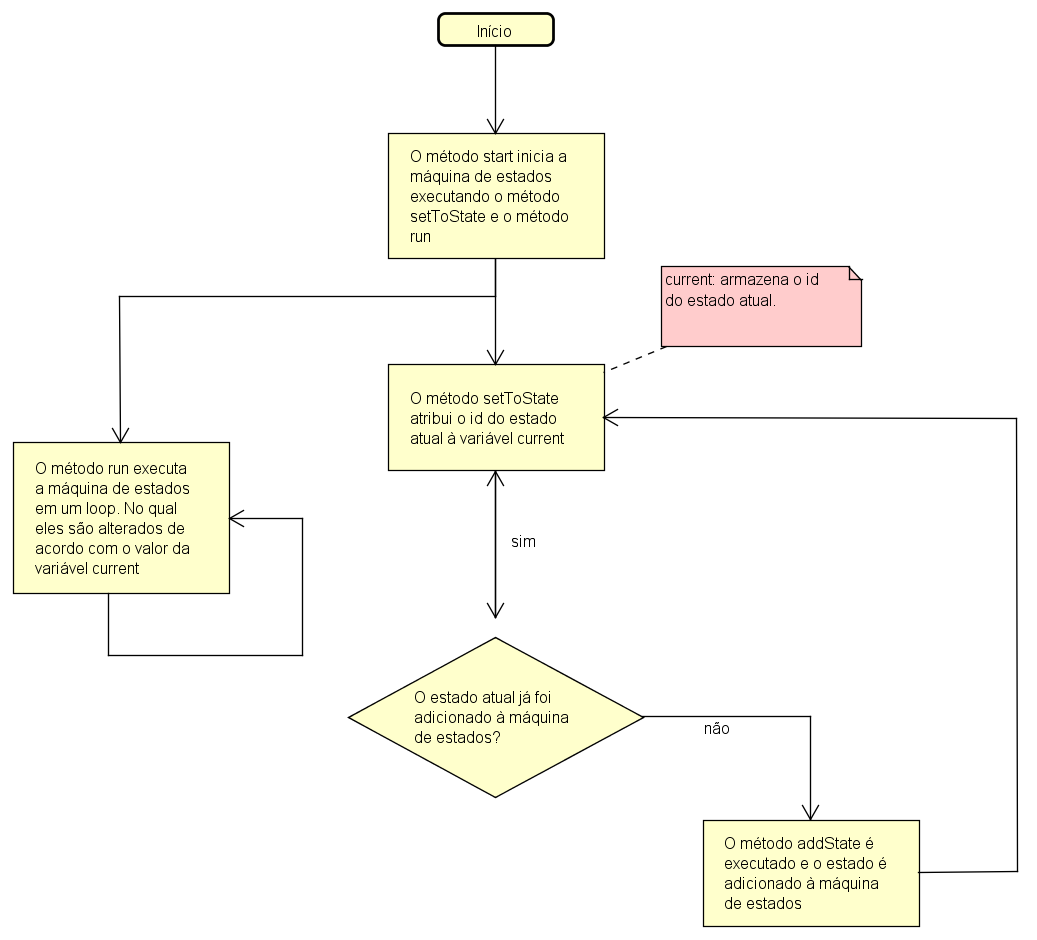
\includegraphics[width=0.6\textwidth]{figuras/fluxoFaultRecovery}\end{center}
		\caption{Fluxograma do funcionamento da máquina de estados da biblioteca.} \label{Fig:fluxoFaultRecovery}
	\end{figure}
\end{frame}

\subsection{Classe de Redundância de Dados: TData}

\begin{frame}
	\frametitle{Classe TData}	
		\begin{itemize}
			\item Redundância de dados automatizada tanto para variáveis primitivas quanto para objetos.
			\item O valor do objeto é armazenado em 3 cópias de segurança.
			\item As cópias são protegidas por um esquema de votação.
			\item Funciona com ponteiros e objetos de pilha.
			\item Mínima reescrita de código.
			\item Exemplo:
			\begin{itemize}
			\item TData$<$tipo\_da\_variável$>$ variavel(valor ou objeto).
			\end{itemize}		
		\end{itemize}		
\end{frame}


%\begin{frame}
%	\frametitle{Processo de leitura dos sensores}
%	\begin{figure}
%		\centering
%		\begin{subfigure}[t]{4.0in}
%			\centering
%			\includegraphics[scale=0.65]{figuras/le_sensores}
%			\caption{Sem injeção de falhas}\label{Fig:LeSensoresOrig}		
%		\end{subfigure}
%		\qquad
%		\begin{subfigure}[t]{4.0in}
%			\centering
%			\includegraphics[scale=0.65]{figuras/le_sensores_injeta_falhas}
%			\caption{Com injeção de falhas.}\label{Fig:InjecaoSensores}
%		\end{subfigure}
%		\caption{Processo de leitura dos sensores na estação meteorológica sem tolerância a falhas}\label{Fig:LeSensores}
%	\end{figure}
%\end{frame}

